\chapter{Principes de base}
\label{chap:bases}

Un système de mise en page tel que {\LaTeX} repose sur une logique de
séparation entre l'apparence d'un document et sa structure. La
personne habituée à utiliser un traitement de texte devra fort
probablement se défaire d'une vilaine habitude: se préoccuper sans
cesse de la disposition du texte au moment de la rédaction.

Ce principe accepté, il faudra néanmoins indiquer au logiciel la
structure du document. Avec {\LaTeX} cela s'effectue par le biais de
diverses instructions que l'on insére au fil du texte. À la base, les
logiciels de traitements de texte n'opèrent pas différemment, sauf
qu'ils cachent les codes aux utilisateurs\footnote{%
  Le leader du traitement de texte jusqu'au milieu des années 1990,
  Word~Perfect, offrait l'option d'afficher l'ensemble des codes de
  mise en page. C'est malheureusement une caractéristique brillante
  que Microsoft Word et les autres progiciels développés depuis ont
  choisi d'omettre.}. %
Sous prétexte de simplicité d'utilisation, ils causent en fait bien
des mots de tête. En utilisant un traitement de texte moderne, vous
vous êtes sans doute déjà demandé: «Pourquoi mon texte est-il
soudainement en gras?»

Ce chapitre explique comment aborder la rédaction d'un document avec
{\LaTeX} ainsi que la syntaxe de base des différents types
d'instructions que l'on peut insérer dans un texte pour en spécifier
la structure et la mise en forme.


\section{Séparation du contenu et de l'apparence}
\label{sec:bases:separation}

Lors de la rédaction avec un système de mise en page tel que {\LaTeX},
on se concentre sur le contenu et la \emph{structure} du document, et
non pas sur son \emph{apparence}. Par exemple:
\begin{itemize}
\item au lieu de prescrire qu'un titre de section doit être en gras
  14~points, on indique simplement à {\LaTeX} que le texte doit être
  traité comme un titre de section;
  \begin{demo}
    \begin{minipage}{0.45\linewidth}
\begin{lstlisting}
\textbf{\large Titre}
\end{lstlisting}
    \end{minipage}
    \hfill \faArrowRight \hfill
    \begin{minipage}{0.45\linewidth}
\begin{lstlisting}
\section{Titre}
\end{lstlisting}
    \end{minipage}
  \end{demo}
\item au lieu de décider qu'un mot sur lequel l'on souhaite insister
  sera en italique, on indique à {\LaTeX} de mettre de l'emphase sur
  ce mot sans se soucier de la mise en forme.
  \begin{demo}
    \begin{minipage}{0.45\linewidth}
\begin{lstlisting}
\textit{texte}
\end{lstlisting}
    \end{minipage}
    \hfill \faArrowRight \hfill
    \begin{minipage}{0.45\linewidth}
\begin{lstlisting}
\emph{texte}
\end{lstlisting}
    \end{minipage}
  \end{demo}
\end{itemize}

L'apparence du texte sera prise en charge par {\LaTeX}. Comme les
gabarits sont l'{\oe}uvre de spécialistes en typographie, il est
généralement préférable de ne pas les modifier. À titre d'exemple,
{\LaTeX} détermine automatiquement la largeur des marges en fonction
de la taille de la police de caractère de manière à ce que les lignes
de texte comptent approximativement 70~caractères. La raison:
lorsqu'une ligne de texte est trop longue, notre {\oe}il a de la
difficulté à la suivre sur toute sa longueur. Il a tendance à passer à
la ligne inférieure, ce qui rend la lecture plus difficile.


\section{Règles de saisie}
\label{sec:bases:saisie}

Une fois le principe de séparation du contenu et de l'apparence
compris et accepté, on veillera, lors de la saisie du texte, à
respecter les règles simples suivantes.
\begin{enumerate}
\item On sépare les mots par une ou plusieurs \emph{espaces}. Qu'il y
  en ait une ou un millier, seule la première compte et la mise en
  page sera la même.
  \begin{demo}
    \begin{texample}
\begin{lstlisting}
Les espaces délimitent les
mots. Leur nombre n'a pas
d'importance.
\end{lstlisting}
      \producing
      Les espaces délimitent les
      mots. Leur nombre n'a pas
      d'importance.
    \end{texample}
    \begin{texample}
\begin{lstlisting}[showstringspaces=true]
Les  espaces   délimitent
les                 mots.
Leur    nombre  n'a pas
d'importance.
\end{lstlisting}
      \producing
      Les  espaces   délimitent
      les                 mots.
      Leur    nombre  n'a pas
      d'importance.
    \end{texample}
  \end{demo}
%
\item On sépare les paragraphes par une ou plusieurs lignes blanches.
  Celles-ci n'apparaîtront pas nécessairement dans le texte final; les
  gabarits standards identifient les paragraphes par un retrait de
  première ligne.
  \begin{demo}
    \begin{texample}
\begin{lstlisting}
Les lignes blanches
délimitent les
paragraphes.

Leur nombre n'a pas
d'importance.
\end{lstlisting}
      \producing
Les lignes blanches
délimitent les
paragraphes.

        Leur nombre n'a pas
        d'importance.
    \end{texample}
\begin{texample}
\begin{lstlisting}
Les lignes blanches
délimitent les
paragraphes.



Leur nombre n'a pas
d'importance.
\end{lstlisting}
      \producing
        Les lignes blanches  délimitent
        les paragraphes.



        Leur nombre n'a pas
        d'importance.
    \end{texample}
  \end{demo}
%
\item On utilise des \emph{commandes} pour indiquer la structure du
  texte dans le code source. Celles-ci débutent presque toujours par
  le caractère {\bs}. À la différence des logiciel de traitement de
  texte, les instructions de mise en forme du document sont donc
  toujours visibles et, par conséquent, modifiables facilement et sans
  surprise (on ne se demande donc jamais où termine le gras).
  \begin{demo}
    \begin{texample}
\begin{lstlisting}
Les commandes sont visibles
dans le \textbf{code source},
mais évidemment pas dans le
\emph{document} fini.
\end{lstlisting}
      \producing
      Les commandes sont visibles
      dans le \textbf{code source},
      mais évidemment pas dans le
      \emph{document} fini.
    \end{texample}
  \end{demo}
\end{enumerate}


\section{Structure d'un fichier}
\label{sec:bases:structure}

Un fichier source {\LaTeX} --- dont on trouvera un exemple simple à la
\autoref{fig:bases:parties} --- est toujours composé de deux parties.

\begin{figure}
  \centering
  \begin{minipage}{0.75\linewidth}
\begin{lstlisting}[numbers=left, numberstyle=\tiny,
                   frame=single, rulecolor=\color{black}, framesep=6pt]
\documentclass[11pt,french]{article} `\label{lst:bases:preambule_debut}'
  \usepackage{babel}
  \usepackage[autolanguage]{numprint}
  \usepackage[utf8]{inputenc}
  \usepackage[T1]{fontenc} `\label{lst:bases:preambule_fin}'

\begin{document} `\label{lst:bases:corps_debut}'

Lorem ipsum dolor sit amet, consectetur
adipiscing elit. Donec quam nulla, bibendum
vitae ipsum vel, fermentum pellentesque orci.

\end{document} `\label{lst:bases:corps_fin}'
\end{lstlisting}
  \end{minipage}
  \caption{Fichier source {\LaTeX} simple comportant les deux parties
    obligatoires: le préambule (lignes
    \ref*{lst:bases:preambule_debut}--\ref*{lst:bases:preambule_fin})
    et le corps du document (lignes
    \ref*{lst:bases:corps_debut}--\ref*{lst:bases:corps_fin}).}
  \label{fig:bases:parties}
\end{figure}

\begin{description}
\item[Préambule] Suite de commandes spécifiant la mise en forme
  globale du document (format du papier, marges, entête et pied de
  page, etc.). Il contient au minimum la commande
  \cmd{\documentclass}. Les commandes contenues dans le préambule ont
  un effet global sur le document.

  Dans l'exemple de la \autoref{fig:bases:parties}, le préambule
  s'étend de la ligne \ref*{lst:bases:preambule_debut} à la ligne
  \ref*{lst:bases:preambule_fin}.
\item[Corps du document] Contenu du document en tant que tel.
  Il débute par \verb=\begin{document}= et se termine par
    \verb=\end{document}=. Le corps du document peut aussi contenir
  des commandes, mais l'effet de celles-ci est presque toujours local.

  Les lignes \ref*{lst:bases:corps_debut}--\ref*{lst:bases:corps_fin}
  du code de la \autoref{fig:bases:parties} forment le corps de ce
  document.
\end{description}


\section{Classes et paquetages}
\label{sec:bases:classes}

La première commande du préambule est normalement la déclaration de la
\emph{classe} du document. La forme de la déclaration est la suivante:
\begin{lstlisting}
\documentclass`\oarg{options}\marg{classe}'
\end{lstlisting}
Les classes standards de {\LaTeX} sont \class{article},
\class{report}, \class{book}, \class{letter} et \class{slides}. La
classe pour les thèses et mémoires de l'Université Laval se nomme
\class{ulthese} \citep{ulthese}. Celle-ci se base sur la classe
\class{memoir} et, par conséquent, hérite de toutes ses (nombreuses)
fonctionnalités; consulter la %
\doc{ulthese}{http://texdoc.net/pkg/ulthese} %
de la classe \class{ulthese} pour les détails. La
\autoref{sec:organisation:classe} revient sur les différences entre les
diverses classes et les \meta{options} disponibles.

Les \emph{paquetages} permettent de modifier des commandes ou
d'ajouter des fonctionnalités à {\LaTeX}. On charge les paquetages
dans le préambule avec des commandes de la forme
\begin{lstlisting}
\usepackage`\marg{paquetage}'
\usepackage`\oarg{options}\marg{paquetage}'
\usepackage`\marg{paquetage1,paquetage2, ...}'
\end{lstlisting}
La première et la troisième forme permettent de charger un ou
plusieurs paquetages sans options. La seconde permet de spécifier des
\meta{options} au chargement du paquetage. Il n'est évidemment pas
possible de préciser des options avec la troisième forme puisque
{\LaTeX} ne saurait à quel paquetage celles-ci se rapportent.

Certains paquetages permettent que leurs options apparaissent parmi
les \meta{options} de la commande \cmdprint{\documentclass}. Elles
sont ainsi plus «visibles» pour d'autres paquetages. Par exemple,
l'option \code{french} que l'on retrouve dans la déclaration de la
classe à la \autoref{fig:bases:parties} est en fait une option du
paquetage \pkg{babel}.

La classe \class{ulthese} charge par défaut un certain nombre de
paquetages essentiels ou incontournables pour la rédaction en
français. Encore ici, consulter la %
\doc{}{http://texdoc.net/pkg/ulthese} %
pour les détails.


\section{Commandes}
\label{sec:bases:commandes}

Nous avons déjà fait référence à quelques reprises au concept de
commande {\LaTeX}. Cette section se penche sur leur syntaxe.

Les formes générales des commandes {\LaTeX} sont:
\begin{lstlisting}
\`\meta{nomcommande}\oarg{arg\_optionnel}\marg{arg\_obligatoire}'
\`\meta{nomcommande}'*`\oarg{arg\_optionnel}\marg{arg\_obligatoire}'
\end{lstlisting}
Ici, \meta{nomcommande} est le nom de la commande. Il débute par le
caractère {\bs} et est exclusivement formé de lettres, habituellement
des minuscules ({\LaTeX} est sensible à la casse). La forme étoilée
d'une commande réalise généralement une action légèrement différente
de la version sans étoile. Par exemple, la commande \cmd{\section}
crée une nouvelle section numérotée, alors que \cmd{\section*}
n'insère aucune numérotation.

Lorsque la commande prend des arguments, les arguments obligatoires
sont placés entre accolades \verb={ }= et les arguments optionnels
sont placés entre crochets \verb=[ ]=.

Certaines commandes n'ont aucun argument. Leur forme est alors
\begin{lstlisting}
\`\meta{nomcommande}
\end{lstlisting}
Dans ce cas, le nom d'une commande se termine par tout caractère qui
n'est pas une lettre --- y compris l'espace! Cette règle fait en sorte
qu'une espace après le nom d'une commande est considéré comme un
marqueur de la fin du nom de celle-ci. Cette règle joue parfois de
vilains tours en «avalant» l'espace entre une commande et le mot qui
suit; voir l'\autoref{exemple:base:commandes} et
l'\autoref{ex:base:commandes}.

La portée d'une commande est limitée à la zone entre accolades
\verb={ }=, le cas échéant.

\begin{exemple}
  \label{exemple:base:commandes}
  Voici trois exemples de commandes {\LaTeX}: une sans argument, une
  avec un seul argument obligatoire et une commande avec deux
  arguments obligatoires et un argument optionnel.
  \begin{enumerate}
  \item La commande \cmd{\LaTeX} permet de composer de logo {\LaTeX}.
    \begin{demo}
      \begin{texample}
\begin{lstlisting}
Apprendre \LaTeX c'est
formidable!
\end{lstlisting}
        \producing
        Apprendre \LaTeX c'est
        formidable!
      \end{texample}
    \end{demo}
    On constate ici l'effet de la règle mentionnée précédemment:
    l'espace suivant le nom de la commande a été interprété par
    {\LaTeX} comme un marqueur de la fin de la commande et il a été
    supprimé du texte. Pour contourner ce problème, nous pouvons soit
    fournir un argument vide à la commande, soit la placer en
    accolades pour limiter sa portée à elle-même:
    \begin{demo}
      \begin{texample}
\begin{lstlisting}
Apprendre \LaTeX{} c'est
formidable!
\end{lstlisting}
        \producing
        Apprendre \LaTeX{} c'est
        formidable!
      \end{texample}
      \begin{texample}
\begin{lstlisting}
Apprendre {\LaTeX} c'est
formidable!
\end{lstlisting}
        \producing
        Apprendre {\LaTeX} c'est
        formidable!
      \end{texample}
    \end{demo}
    %
  \item La commande \cmd{\emph} met de l'emphase (en général sous
    forme d'italique) sur le ou les mots en argument.
    \begin{demo}
      \begin{texample}
\begin{lstlisting}
Il est \emph{essentiel} de
connaître la syntaxe de
{\LaTeX}.
\end{lstlisting}
        \producing
        Il est \emph{essentiel} de
        connaître la syntaxe de
        {\LaTeX}.
      \end{texample}
    \end{demo}
    %
  \item La commande \cmd{\rule} produit un rectangle plein. Elle a
    deux arugments obligatoires: la longueur et la hauteur du
    rectangle, dans l'ordre. Un argument optionnel permet de surélever
    le rectangle au-dessus de la ligne de base (voir le
    \autoref{chap:boites} pour plus de détails).
    \begin{demo}
      \begin{texample}
\begin{lstlisting}
Réglure de 1~cm de long et
3~mm d'épais surélevée de
2~points au-dessus de la
ligne de base:
\rule[2pt]{1cm}{3mm}.
\end{lstlisting}
        \producing
        Réglure de $1$~cm de long et
        $3$~mm d'épais surélevée de
        $2$~points au-dessus de la
        ligne de base: \rule[2pt]{1cm}{3mm}.
      \end{texample}
    \end{demo}
  \end{enumerate}
  \qed
\end{exemple}

\begin{exemple}
  La commande \cmd{\bfseries} sélectionne une police de caractère
  grasse pour tout le texte qui suit.
  \begin{demo}
    \begin{texample}
\begin{lstlisting}
En typographie, la \bfseries
graisse est l'épaisseur d'un
trait ou d'un caractère.
\end{lstlisting}
      \producing
      En typographie, la \bfseries
      graisse est l'épaisseur d'un
      trait ou d'un caractère.
    \end{texample}
  \end{demo}
  Pour limiter le changement à une zone de texte, il faut la délimiter
  par des accolades.
\begin{demo}
    \begin{texample}
\begin{lstlisting}
En typographie, la {\bfseries
graisse est l'épaisseur d'un
trait} ou d'un caractère.
\end{lstlisting}
      \producing
      En typographie, la {\bfseries
      graisse est l'épaisseur d’un
      trait} ou d’un caractère.
    \end{texample}
  \end{demo}
  \qed
\end{exemple}

L'usager de {\LaTeX} peut définir de nouvelles commandes à loisir.
Ceci est expliqué à la \autoref{sec:commandes:commandes}.


\section{Environnements}
\label{sec:bases:environnements}

Un environnement {\LaTeX} est simplement une zone de texte délimitée
par une construction du type
\begin{lstlisting}
\begin`\marg{environnement}'
   ...
\end`\marg{environnement}'
\end{lstlisting}
Le contenu d'un environnement est traité différemment du reste du
texte en fonction des paramètres de l'environnement. Par exemple, le
texte à l'intérieur d'un environnement \Ie{center} est centré sur la
page.

Les changements induits par un environnement s'appliquent uniquement à
l'intérieur de celui-ci. Il en va de même des commandes utilisées à
l'intérieur d'un environnement.

\begin{exemple}
  L'environnement \Ie{quote} sert à composer des citations. Le texte à
  l'intérieur de l'environnement sera placé dans un bloc séparé du
  texte principal et en retrait des marges gauche et droite.
  \begin{demo}
    \begin{texample}
\begin{lstlisting}
La phrase
\begin{quote}
  Attention aux bogues dans le
  code ci-dessus; je ne l'ai
  pas testé, j'ai seulement
  prouvé qu'il était correct.
\end{quote}
est une citation célèbre du
créateur de {\TeX}, Donald
Knuth.
\end{lstlisting}
      \producing
      La phrase
      \begin{quote}
        Attention aux bogues dans le code ci-dessus; je ne l'ai pas testé,
        j'ai seulement prouvé qu'il était correct.
      \end{quote}
      est une citation célèbre du créateur de {\TeX}, Donald Knuth.
    \end{texample}
  \end{demo}
  Si la citation est dans la langue originale, il est préférable de la
  composer en italique.
  \begin{demo}
    \begin{texample}
\begin{lstlisting}
La phrase
\begin{quote}
  \itshape
  Beware of bugs in the above
  code; I have only proved it
  correct, not tried it.
\end{quote}
est une citation célèbre du
créateur de {\TeX}, Donald
Knuth.
\end{lstlisting}
      \producing
      La phrase
      \begin{quote}
        \itshape
        Beware of bugs in the above code; I have only proved it
        correct, not tried it.
      \end{quote}
      est une citation célèbre du créateur de {\TeX}, Donald Knuth.
    \end{texample}
  \end{demo}
  On remarque que l'effet de la commande \cmdprint{\itshape} s'est
  limité à l'environnement. %
  \qed
\end{exemple}


\section{Longueurs}
\label{sec:bases:longueurs}

Plusieurs commandes {\LaTeX} requièrent en argument une mesure de
largeur ou de hauteur. Dans la terminologie de {\LaTeX}, on parle plus
généralement de longueur\index{longueur} (\emph{length}).

Une longueur est un nombre positif, négatif ou nul
\emph{obligatoirement} et \emph{immédiatement} suivi d'un symbole
d'unité de mesure. Le \autoref{tab:bases:longueurs} présente les
principales unités de mesure utilisées par {\LaTeX} et le symbole
correspondant.

\begin{table}
  \caption{Principales unités de mesure pour les longueurs dans
    {\LaTeX}}
  \label{tab:bases:longueurs}
  \centering
  \begin{tabular}{lcl}
    \toprule
    nom ou description & symbole & longueur équivalente \\
    \midrule
    millimètre & \texttt{mm} \\
    centimètre & \texttt{cm} & $10$~mm \\
    pouce      & \texttt{in} & $2,54$~cm \\
    point      & \texttt{pt} & $1/72,27$~pouce \\
    point PostScript     & \texttt{bp}   & $1/72$~pouce \\
    largeur de la lettre M & \texttt{em} & fonction de la police \\
    hauteur de la lettre x & \texttt{ex} & fonction de la police \\
    \bottomrule
  \end{tabular}
\end{table}

Il existe un certain nombre de longueurs prédéfinies. Les plus utiles
sont:
\begin{lstlisting}
\linewidth
\textwidth
\end{lstlisting}
La première contient la largeur de la ligne de texte courante et la
seconde, la largeur de la page courante. Dans du texte normal, les
deux mesures sont habituellement égales.


\section{Caractères spéciaux}
\label{sec:bases:caracteres}

Les claviers d'ordinateur mettent à la disposition des auteurs toutes
les lettres de l'alphabet (en versions minuscule et majuscule), les
chiffres de 0 à 9, un certain nombre de symboles et, selon le clavier,
des versions accentuées de certaines lettres. L'entrée des lettres et
des chiffres ne pose pas de problème particulier pour {\LaTeX}, mais
certains symboles sont reservés. De plus, certains symboles d'usage
courant ne sont pas disponibles sur les claviers.

\subsection{Espaces et retours à la ligne}
\label{sec:bases:caracteres:espaces}

Nous avons déjà mentionné à la \autoref{sec:bases:saisie} le
traitement spécial réservé par {\LaTeX} aux espaces et aux retours à
la ligne dans le code source. Ajoutons des précisions suivantes:
\begin{itemize}
\item seule la première espace entre deux éléments compte;
\item les espaces en début de ligne sont ignorées;
\item un retour à la ligne simple est traité comme une espace;
\item il faut deux retours à la ligne consécutifs (ce qui résulte en
  une ligne blanche dans le code source) pour identifier un changement
  de paragraphe.
\end{itemize}

Pour forcer une espace à un endroit où {\LaTeX} la supprimerait
normalement, utiliser la commande \verb*=\ = (le symbole \bs\ suivi
d'une espace, représentée ici par le symbole \verb*| |.
\begin{demo}
  \begin{texample}
\begin{lstlisting}
Apprendre \LaTeX\ c'est
formidable!
\end{lstlisting}
    \producing
    Apprendre \LaTeX\ c'est
    formidable!
  \end{texample}
\end{demo}

Il arrive que l'espace générée par un retour à la ligne \emph{simple}
s'avère indésirable. Dans de tels cas, placer un symbole de
commentaire \verb=%= à la fin de la ligne.
\begin{demo}
  \begin{texample}
\begin{lstlisting}
Donald Knuth est un dieu
\textsuperscript{[citation]}
.
\end{lstlisting}
    \producing
    Donald Knuth est un dieu
    \textsuperscript{[citation]}
    .
  \end{texample}
  \begin{texample}
\begin{lstlisting}
Donald Knuth est un dieu%
\textsuperscript{[citation]}%
.
\end{lstlisting}
    \producing
    Donald Knuth est un dieu%
    \textsuperscript{[citation]}%
    .
  \end{texample}
\end{demo}

\subsection{Caractères réservés}
\label{sec:bases:caracteres:reserves}

Comme à peu près tous les langages de programmation, {\TeX} réserve
certains symboles pour son usage interne. Les symboles suivants sont
interprétés comme des commandes:
\begin{center}
  \verb=# $ & ~ _ ^ % { }=
\end{center}
Pour utiliser ces symboles tels quels dans le texte, il faut les
précéder par le caractère {\bs}:
\begin{demo}
  \begin{minipage}{0.2\linewidth}
    \begin{texample}
\begin{lstlisting}
\#
\end{lstlisting}
      \producing\ \#
    \end{texample}
  \end{minipage}
  \hfill
  \begin{minipage}{0.2\linewidth}
    \begin{texample}
\begin{lstlisting}
\$
\end{lstlisting}
      \producing\ \$
    \end{texample}
  \end{minipage}
  \hfill
  \begin{minipage}{0.2\linewidth}
    \begin{texample}
\begin{lstlisting}[commentstyle=\mdseries]
\%
\end{lstlisting}
      \producing\ \%
    \end{texample}
  \end{minipage}
  \\
  \begin{minipage}{0.2\linewidth}
    \begin{texample}
\begin{lstlisting}
\_
\end{lstlisting}
      \producing\rule{0pt}{1em}\ \_
    \end{texample}
  \end{minipage}
  \hfill
  \begin{minipage}{0.2\linewidth}
    \begin{texample}
\begin{lstlisting}
\{
\end{lstlisting}
      \producing\ \}
    \end{texample}
  \end{minipage}
  \hfill
  \begin{minipage}{0.2\linewidth}
    \begin{texample}
\begin{lstlisting}
\}
\end{lstlisting}
      \producing\ \}
    \end{texample}
  \end{minipage}
\end{demo}

\subsection{Guillemets}
\label{sec:bases:caracteres:guillemets}

L'usage des guillemets nécessite une attention particulière dans
{\LaTeX}. On ne devrait pas utiliser dans le code source les
guillemets doubles (\verb="=) que l'on trouve couramment sur les
claviers d'ordinateurs.

Pour obtenir les guillemets anglais, on utilisera deux symboles
d'accent grave côte-à-côte pour les guillemets ouvrants (``) et deux
apostrophes côte-à-côte pour les guillemets fermants ('').
\begin{demo}
  \begin{texample}
\begin{lstlisting}[escapeinside={}]
``guillemets anglais''
\end{lstlisting}
    \producing
    ``guillemets anglais''
  \end{texample}
\end{demo}

En typographie française, il convient d'utiliser les chevrons («\ »)
comme guillemets. Avec la configuration appropriée de \pkg{babel}
(voir la \autoref{sec:bases:francais}), il suffit d'utiliser dans le
code source les symboles \,\verb=«=\, et \,\verb=»=\, que l'on
retrouve normalement sur un clavier français. L'espacement requis
autour des symboles est géré automatiquement.
\begin{demo}
  \begin{texample}
\begin{lstlisting}
«guillemets français»
\end{lstlisting}
    \producing
    «guillemets français»
  \end{texample}
  \begin{texample}
\begin{lstlisting}
« guillemets français »
\end{lstlisting}
    \producing
    « guillemets français »
  \end{texample}
\end{demo}
Les guillemets anglais ne servent, en français, que pour les citations
incluses, c'est-à-dire pour les citations à l'intérieur d'une
citation.
\begin{demo}
  \begin{texample}
\begin{lstlisting}[escapeinside={}]
Elle m'a dit: «Laurent fait
dire ``non merci''.»
\end{lstlisting}
    \producing
    Elle m'a dit: «Laurent fait
    dire ``non merci''.»
  \end{texample}
\end{demo}

Les bons éditeurs de texte adaptés pour {\LaTeX} redéfinissent
l'action de la touche \fbox{\texttt{\textquotedbl}} du clavier pour
insérer les symboles appropriés selon la langue du document.

Le paquetage \pkg{csquotes} \citep{csquotes} propose une autre option
pour l'entrée des guillemets. Il fournit une commande
\cmdprint{\enquote} qui entoure son argument des guillemets appropriés
selon le contexte et la langue du texte. Cette solution peut s'avérer
intéressante pour les nouveaux venus à {\LaTeX} qui n'ont pas encore
pris l'habitude d'entrer directement les bons guillemets.

\subsection{Trait d'union et tirets}
\label{sec:bases:caracteres:tirets}

On trouve en typographie soignée trois sortes de tirets de longueurs
différentes:
\begin{enumerate}
\item le trait d'union (-) qui sert à relier des mots entre eux;
\item le tiret demi-cadratin (--) qui sert à joindre deux éléments qui
  comportent déjà des traits d'union (\emph{Trois-Rivières--Québec});
\item le tiret cadratin (---) qui sert à identifier le changement
  d'interlocuteur dans les dialogues ou qui remplacent parfois les
  parenthèses dans du texte normal.
\end{enumerate}

S'il est simple d'entrer un trait d'union à l'ordinateur, il est rare
que les claviers comportent des touches pour entrer les tirets
demi-cadratin et cadratin (ou alors cela se fait via une obscure
combinaison de touches). {\LaTeX} permet de créer facilement tous les
tirets ci-dessus en répétant simplement le trait d'union deux ou trois
fois.
\begin{demo}
  \begin{minipage}{0.2\linewidth}
    \begin{texample}
\begin{lstlisting}
-
\end{lstlisting}
      \producing\ -
    \end{texample}
  \end{minipage}
  \hfill
  \begin{minipage}{0.2\linewidth}
    \begin{texample}
\begin{lstlisting}
--
\end{lstlisting}
      \producing\ --
    \end{texample}
  \end{minipage}
  \hfill
  \begin{minipage}{0.2\linewidth}
    \begin{texample}
\begin{lstlisting}
---
\end{lstlisting}
      \producing\ ---
    \end{texample}
  \end{minipage}
\end{demo}

\subsection{Accents et ligatures}
\label{sec:bases:caracteres:accents}

À la base, {\LaTeX} ne reconnait pas les lettres accentuées ni les
ligatures comme {\ae} et {\oe} qui ne sont pas courantes en anglais.
Néanmoins, il est possible de créer ces symboles avec des commandes.
\begin{demo}
  \begin{minipage}{0.2\linewidth}
    \begin{texample}
\begin{lstlisting}
\'{o}
\end{lstlisting}
      \producing\ \'{o}
    \end{texample}
  \end{minipage}
  \hfill
  \begin{minipage}{0.2\linewidth}
    \begin{texample}
\begin{lstlisting}[escapeinside={}]
\`{o}
\end{lstlisting}
      \producing\ \`{o}
    \end{texample}
  \end{minipage}
  \hfill
  \begin{minipage}{0.2\linewidth}
    \begin{texample}
\begin{lstlisting}
\^{o}
\end{lstlisting}
      \producing\ \^{o}
    \end{texample}
  \end{minipage}
  \hfill
  \begin{minipage}{0.2\linewidth}
    \begin{texample}
\begin{lstlisting}
\"{o}
\end{lstlisting}
      \producing\ \"{o}
    \end{texample}
  \end{minipage} \\
  \hfill
  \begin{minipage}{0.2\linewidth}
    \begin{texample}
\begin{lstlisting}
{\ae}
\end{lstlisting}
      \producing\ \ae
    \end{texample}
  \end{minipage}
  \hfill
  \begin{minipage}{0.2\linewidth}
    \begin{texample}
\begin{lstlisting}
{\AE}
\end{lstlisting}
      \producing\ \AE
    \end{texample}
  \end{minipage}
  \hfill
  \begin{minipage}{0.2\linewidth}
    \begin{texample}
\begin{lstlisting}
{\oe}
\end{lstlisting}
      \producing\ \oe
    \end{texample}
  \end{minipage}
  \hfill
  \begin{minipage}{0.2\linewidth}
    \begin{texample}
\begin{lstlisting}
{\OE}
\end{lstlisting}
      \producing\ \OE
    \end{texample}
  \end{minipage}
\end{demo}

Évidemment, entrer tous les accents d'un texte en français avec les
commandes ci-dessus se révélerait un véritable cauchemar.
Heureusement, avec la configuration appropriée, il est possible
d'entrer directement les lettres accentuées que l'on trouve couramment
sur un clavier, voire même certaines ligatures si l'on utilise
l'encodage UTF-8. La \autoref{sec:bases:francais} fournit les détails.

Les commandes pour les accents demeurent utiles pour composer les
lettres accentuées des langues européennes autres que le français. On
trouvera la liste de ces commandes, ainsi que celles pour composer une
multitude d'autres symboles à la section~2 de la très utile %
\doc[Comprehensive {\LaTeX} Symbol
List]{compre\-hen\-sive}{http://texdoc.net/pkg/comprehensive} %
\citep{comprehensive}.


\section{{\LaTeX} en français}
\label{sec:bases:francais}

Par défaut, LaTeX prévoit la rédaction de documents en anglais.
L'entrée de texte en français de façon simple et conviviale requiert
de charger quelques paquetages bien choisis. Le choix dépend lui-même
du moteur {\TeX} utilisé.

\subsection{Moteur pdf\TeX}
\label{sec:bases:francais:pdftex}

Afin de pouvoir entrer directement les lettres accentuées dans le code
source sans avoir recours aux commandes de la section précédente, il
faut s'assurer que les lettres accentuées soient reconnues par
{\LaTeX}. C'est le rôle du paquetage \pkg{inputenc} \citep{inputenc}.
Il faut spécifier le type de codage utilisé, ce qui parfois demande
quelques essais et erreurs. Le type de codage le plus universel en ce
moment est l'Unicode \citep{Unicode:5.0}. C'est le type utilisé par
défaut dans macOS et les distributions Linux; il est aussi
disponible sous Windows. Si le fichier source est sauvegardé dans le
format %
\link{https://fr.wikipedia.org/wiki/UTF-8}{UTF-8} %
de l'Unicode, on ajoutera dans le préambule la commande:
\begin{lstlisting}
\usepackage[utf8]{inputenc}
\end{lstlisting}

Les autres types de codage les plus répandus sont
l'\link{http://fr.wikipedia.org/wiki/Iso_8859-1}{ISO 8859-1}, ou
Latin-1, et l'\link{http://fr.wikipedia.org/wiki/Windows-1252}{ANSI}
de Windows. Pour utiliser ces types, on remplacera \code{utf8}
ci-dessus par, respectivement, \code{latin1} ou \code{ansiwin}.

L'entrée du texte n'est pas tout, il faut également se soucier de la
sortie, afin que les lettres accentuées apparaissent dans le document
final. {\LaTeX} utilise par défaut un codage de sortie des caractères
nommé OT1. Il est recommandé de ne pas utiliser ce codage pour les
textes en français, notamment parce que la césure automatique ne
fonctionnera pas pour les mots contenant des lettres accentuées. On
préférera donc le plus récent codage T1, que l'on active avec le
paquetage \pkg{fontenc} \citep{fontenc}:
\begin{lstlisting}
\usepackage[T1]{fontenc}
\end{lstlisting}

La classe \class{ulthese} charge par défaut le paquetage \pkg{fontenc}
avec l'option T1 et les gabarits de documents fournis avec la classe
contiennent l'instruction pour charger \pkg{inputenc}.

\subsection{Moteur \XeTeX}
\label{sec:bases:francais:xetex}

Le plus récent et moderne moteur {\XeTeX} utilise par défaut des
fichiers source en format Unicode UTF-8. Il n'y a donc rien de spécial
à faire pour l'entrée du texte avec ce moteur.

Pour la sortie, le paquetage \pkg{fontspec} \citep{fontspec} est
requis pour obtenir les lettres accentuées dans le fichier PDF. Cela ne
représente pas véritablement une étape de configuration additionnelle
puisque l'on charge normalement ce paquetage avec {\XeLaTeX} pour
contrôler le chargement des polices de caractères (plus de détails à
la \autoref{sec:trucs:police}).

La classe \class{ulthese} charge par défaut le paquetage
\pkg{fontspec} avec {\XeLaTeX}.

\subsection{Typographie et mots clés français}
\label{sec:bases:francais:babel}

Entrer du texte en français dans le code source n'est pas tout. Il
faut adapter {\LaTeX} au français, qu'il s'agisse des mots clés (tels
«Table des matières» ou «Bibliographie»), de la typographie ou de la
césure des mots. La solution standard provient du paquetage
\pkg{babel} \citep{babel}. Celui-ci permet de combiner plusieurs
langues dans un même document et de passer de l'une à l'autre
facilement. Consulter la %
\doc{frenchb}{http://texdoc.net/pkg/babel-french/} %
pour connaître toutes les adaptations au français offertes par ce
paquetage incontournable.

Le paquetage \pkg{babel} est chargé par défaut par la classe
\class{ulthese}.

\subsection{Guillemets français}
\label{sec:bases:francais:guillemets}

Une espace fine devrait séparer les guillemets du ou des mots qu'ils
entourent. Pour que l'espace autour des symboles soit géré
automatiquement par \pkg{babel}, il suffit d'ajouter dans le préambule
la commande
\begin{lstlisting}
\frenchbsetup{og=«, fg=»}
\end{lstlisting}
On trouve cette configuration dans les gabarits livrés avec la classe
\class{ulthese}.

\subsection{Séparateur décimal}
\label{sec:bases:francais:virgule}

Le séparateur décimal en français est la virgule et non le point. Or,
en mode mathématique, LaTeX ajoute automatiquement une espace fine
après une virgule comme s'il s'agissait d'une énumération.

Afin de pouvoir utiliser de manière conviviale la virgule comme
séparateur décimal en mode mathématique, on chargera le très pratique
paquetage \pkg{icomma} \citep{icomma}. Avec ce paquetage, la virgule
agira comme séparateur décimal en mode mathématique seulement
lorsqu'elle est suivie d'un caractère autre que l'espace.
\begin{demo}
  \begin{minipage}{0.5\linewidth}
    \begin{texample}[0.6\linewidth]
\begin{lstlisting}
% nombre décimal
$x = 1,2$
\end{lstlisting}
      \producing
      $x = 1,2$
    \end{texample}
  \end{minipage}
  \hfill
  \begin{minipage}{0.5\linewidth}
    \begin{texample}[0.6\linewidth]
\begin{lstlisting}
% énumération
$x = 1, 2, 3$
\end{lstlisting}
      \producing
      $x = 1, 2, 3$
    \end{texample}
  \end{minipage}
\end{demo}

\begin{important}
  Le paquetage \pkg{icomma} peut interagir avec d'autres. Aussi
  vaut-il mieux le charger parmi les derniers dans le préambule, et
  certainement après les paquetages \pkg{fontspec} et
  \pkg{unicode-math} avec {\XeLaTeX}.
\end{important}

\subsection{Séparateur des milliers}
\label{sec:bases:francais:milliers}

Le séparateur des milliers en français est l'espace. Lorsque le
paquetage \pkg{numprint} \citep{numprint} est chargé, \pkg{babel}
fournit la commande \cmd{\nombre} pour formater automatiquement les
nombres.
\begin{demo}
  \begin{texample}
\begin{lstlisting}
\nombre{123456789}
\end{lstlisting}
    \producing
    \nombre{123456789}
  \end{texample}
\end{demo}

Le \autoref{tab:bases:francais} résume les divers enjeux liés à la
rédaction en français avec {\LaTeX} et les paquetages qui offrent des
solutions.

\begin{table}
  \centering
  \caption{Enjeux de rédaction en français et paquetages offrant des
    solutions}
  \label{tab:bases:francais}
  \begin{tabularx}{1.0\linewidth}{Xl}
    \toprule
    Enjeu & Solution \\
    \midrule
    \addlinespace[0.5\normalbaselineskip]
    Traduction des mots clés prédéfinis & \pkg{babel} \\
    \addlinespace[0.5\normalbaselineskip]
    Coupure de mots & \pkg{babel} \\
    \addlinespace[0.5\normalbaselineskip]
    Typographie française & \pkg{babel} \\
    \addlinespace[0.5\normalbaselineskip]
    Lettres accentuées dans source & \pkg{inputenc} (\LaTeX) \\
                                   & source en UTF-8 (\XeLaTeX) \\
    \addlinespace[0.5\normalbaselineskip]
    Lettres accentuées dans sortie & \pkg{fontenc} (\LaTeX) \\
                                   & \pkg{fontspec} (\XeLaTeX) \\
    \addlinespace[0.5\normalbaselineskip]
    Virgule comme séparateur décimal & \pkg{icomma} \\
    \addlinespace[0.5\normalbaselineskip]
    Espace comme séparateur des milliers & \pkg{numprint} et
                                           \pkg{babel} \\
    \bottomrule
  \end{tabularx}
\end{table}


%%%
%%% Exercices
%%%

\section{Exercices}
\label{sec:bases:exercices}

\begin{exercice}[nosol]
  Utiliser le fichier \fichier{exercice\_minimal.tex}.
  \begin{enumerate}
  \item Compiler le document avec la classe \class{article}, puis avec
    la classe \class{book}. Observer le résultat.
  \item Ajouter du texte en français (avec accents) et observer le
    résultat.
  \end{enumerate}
\end{exercice}

\begin{exercice}
  \label{ex:base:commandes}
  Modifier le fichier \fichier{exercice\_commandes.tex} afin
  de produire le texte ci-dessous.
  \begin{center}
    \fbox{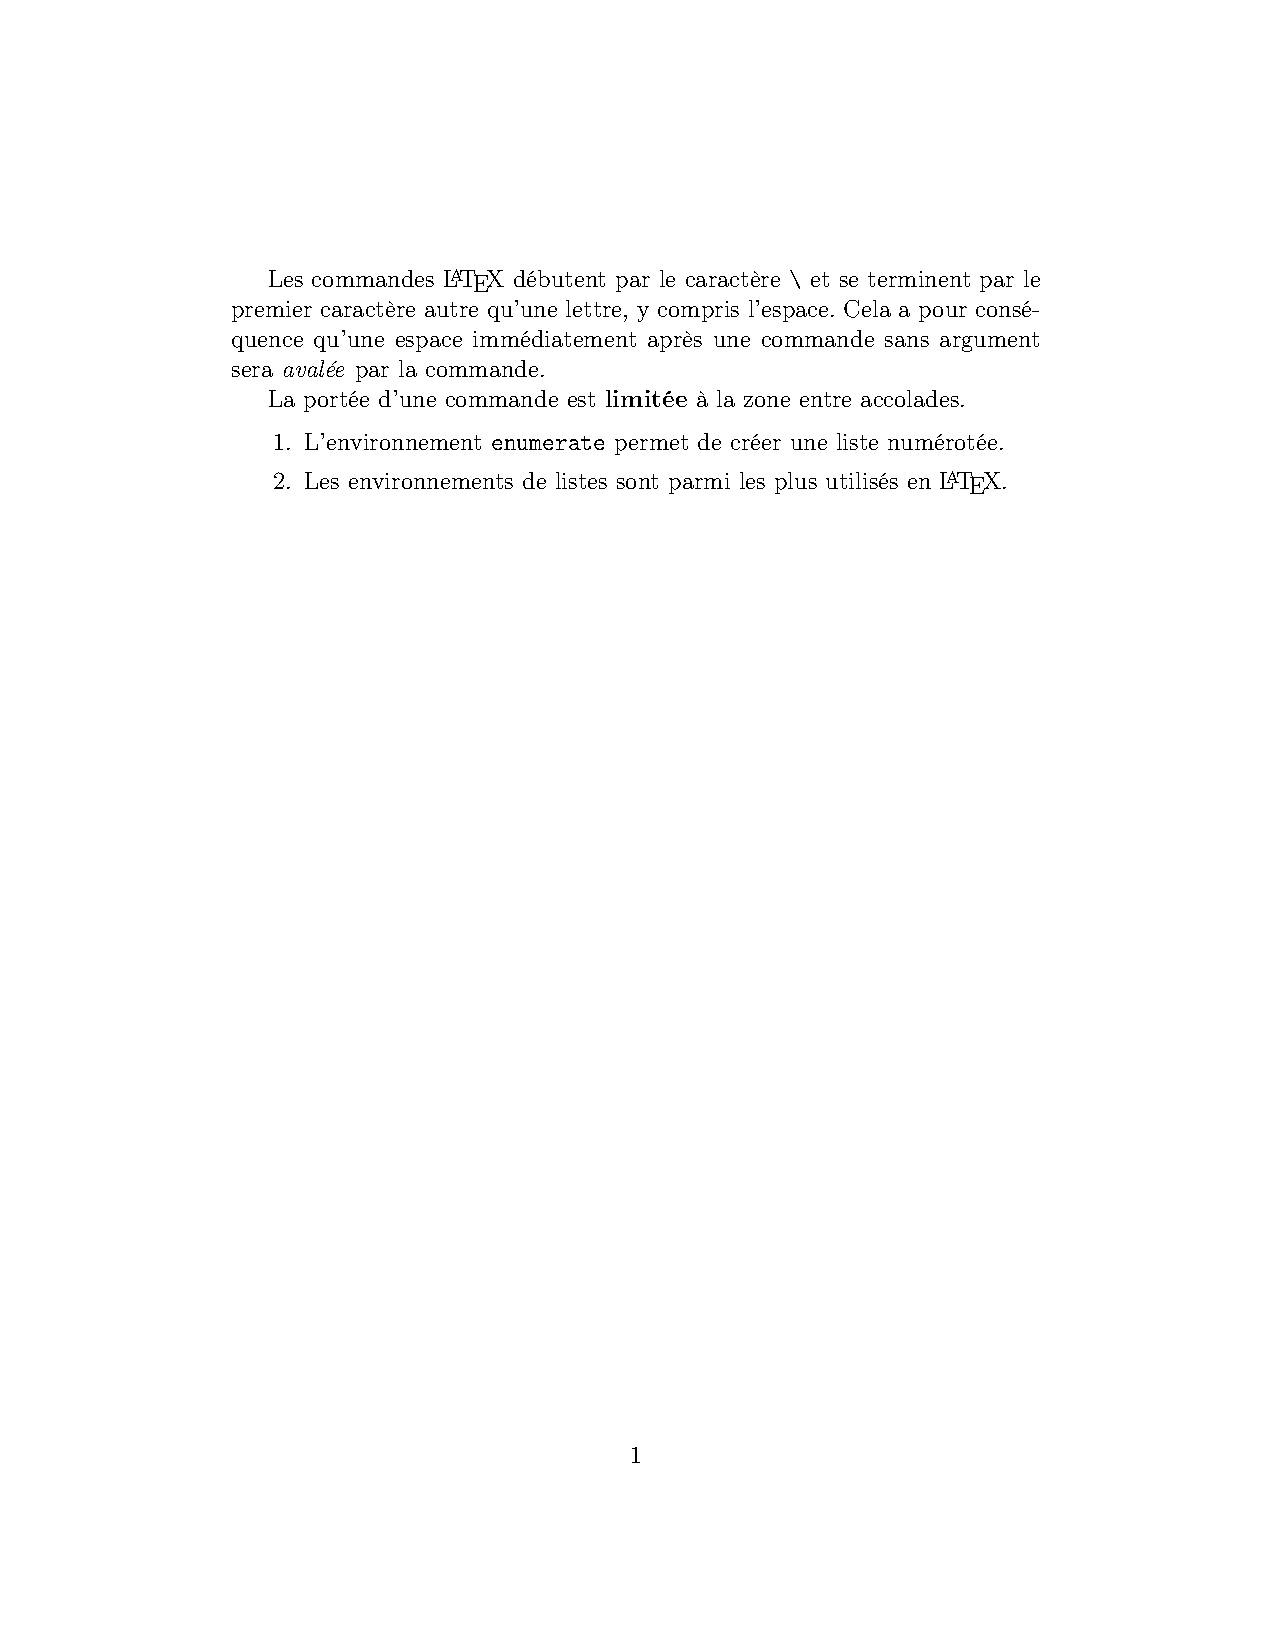
\includegraphics[viewport=108 551 502
      665,width=\linewidth]{exercice_commandes-solution}}
  \end{center}
  \begin{sol}
    Consulter le fichier \fichier{exercice\_commandes-solution.tex}.
  \end{sol}
\end{exercice}

\begin{exercice}
  \begin{enumerate}
  \item Compiler tel que fourni le fichier
    \fichier{exercice\_classe+paquetages.tex}.
  \item Changer la police de caractère du document pour 11~points,
    puis 12~points. Changer la classe du document pour \class{memoir}.
    Observer l'effet sur les marges et sur la coupure automatique des
    mots.
  \item Charger le paquetage \pkg{icomma} et observer l'effet sur la
    formule mathématique.
  \item Charger le paquetage \pkg{numprint} avec l'option
    \verb=autolanguage= (\emph{après} le paquetage \pkg{babel}). Dans
    le code source de la formule mathématique, changer
\begin{lstlisting}
10 000
\end{lstlisting}
    pour
\begin{lstlisting}
\nombre{10000}
\end{lstlisting}
    et observer le résultat.
  \end{enumerate}
  \begin{sol}
    Consulter le fichier \fichier{exercice\_classe+paquetages-solution.tex}.
  \end{sol}
\end{exercice}


%%% Local Variables:
%%% mode: latex
%%% TeX-engine: xetex
%%% TeX-master: "formation-latex-ul"
%%% coding: utf-8
%%% End:
